\documentclass[12pt, a4paper]{article}

\usepackage{amsmath, amsthm, amssymb}
\usepackage{geometry}
\usepackage{hyperref}
\usepackage{enumitem}
\usepackage{booktabs}
\usepackage{array}
\usepackage{xcolor}
\usepackage{parskip}
\usepackage{tikz}
\usetikzlibrary{arrows.meta, positioning, decorations.pathreplacing, calc}

\geometry{margin=2.5cm}
\hypersetup{colorlinks=true, linkcolor=blue!60!black, urlcolor=blue!60!black}

\theoremstyle{definition}
\newtheorem{definition}{Definition}[section]
\newtheorem{theorem}{Theorem}[section]
\newtheorem{lemma}{Lemma}[section]
\newtheorem{proposition}{Proposition}[section]
\newtheorem{corollary}{Corollary}[section]
\newtheorem{remark}{Remark}[section]
\newtheorem{assumption}{Assumption}[section]
\newtheorem{example}{Example}[section]

\newcommand{\E}{\mathbb{E}}
\newcommand{\R}{\mathbb{R}}
\newcommand{\Var}{\mathrm{Var}}
\newcommand{\Cov}{\mathrm{Cov}}
\newcommand{\Prob}{\mathbb{P}}
\newcommand{\borel}{\mathcal{B}}
\newcommand{\sF}{\mathcal{F}}
\newcommand{\sG}{\mathcal{G}}
\newcommand{\expit}{\mathrm{expit}}
\newcommand{\logit}{\mathrm{logit}}
\newcommand{\Leb}{\mathrm{Leb}}
\newcommand{\Range}{\mathrm{Range}}

\title{\textbf{Foundations of Generalised Linear Models, v10}\\
\large From Conditional Expectation to Logistic Regression}
\author{B.~Garbuzov\\[4pt]
{\small Technical notes, 2026}}
\date{}

\begin{document}
\maketitle
\tableofcontents
\newpage

%------------------------------------------------------------
\section{Two approaches to the regression function}
%------------------------------------------------------------

Let $(\Omega, \sF, \Prob)$ be a probability space and
$(X, Y) : \Omega \to \R^2$ a random vector with $\E|Y| < \infty$.

%------------------------------------------------------------
\subsection{Motivation: the discrete case}
%------------------------------------------------------------

Suppose $X$ takes values $x_1, x_2, \ldots$ with $\Prob(X=x_i)>0$.
The sets $A_i = \{X=x_i\}$ are the \emph{atoms} of $\sigma(X)$.

\begin{lemma}[Measurable functions are constant on atoms]
\label{lem:atoms}
Let $A \in \mathcal{S}$ be an atom of a sub-$\sigma$-algebra
$\mathcal{S} \subseteq \sF$.
If $f:\Omega\to\R$ is $\mathcal{S}$-measurable, then $f$ is
$\Prob$-a.e.\ constant on $A$.
\end{lemma}

\begin{proof}
For any $t$, $\{f\leq t\}\cap A\in\mathcal{S}$.
Since $A$ is an atom, its $\Prob$-measure is either $0$ or $\Prob(A)$.
Hence the conditional distribution of $f$ on $A$ is a point mass,
i.e.\ $f=c$ $\Prob$-a.e.\ on $A$ for some $c\in\R$.
\end{proof}

\begin{remark}
For $\sigma(X)$ the atoms are the level sets $A_i=\{X=x_i\}$.
Lemma~\ref{lem:atoms} says $\tilde h(X(\cdot))$ is constant on each
$A_i$, so $h(x_i)=\E[Y\mid X=x_i]$ is a well-defined single number.
\end{remark}

\bigskip
\begin{center}
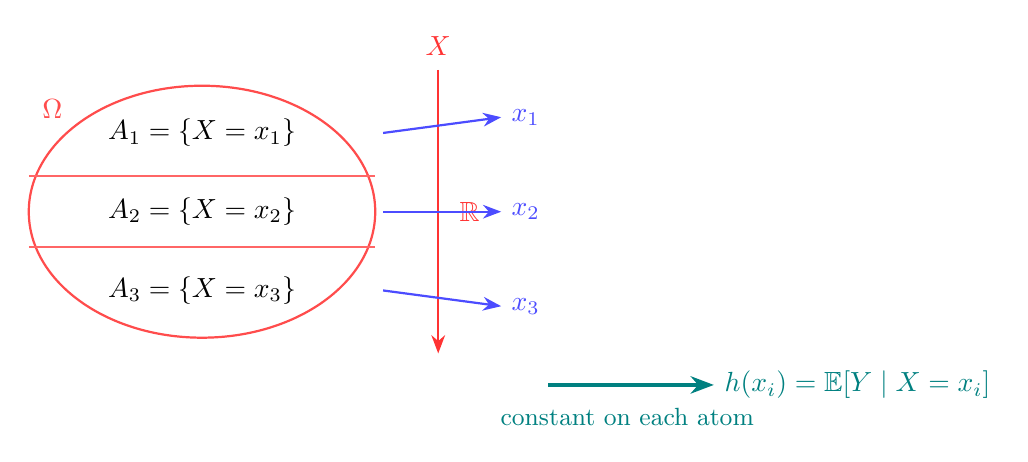
\begin{tikzpicture}[>=Stealth]
  \draw[red!70, thick] (0,0) ellipse (2.2cm and 1.6cm);
  \node[red!70] at (-1.9,1.3) {$\Omega$};
  \draw[red!60,thick] (-2.2,0.45)--(2.2,0.45);
  \draw[red!60,thick] (-2.2,-0.45)--(2.2,-0.45);
  \node at (0, 1.0) {$A_1=\{X=x_1\}$};
  \node at (0, 0.0) {$A_2=\{X=x_2\}$};
  \node at (0,-1.0) {$A_3=\{X=x_3\}$};
  \draw[->,thick,red!80] (3.0,1.8)--(3.0,-1.8)
    node[midway,right=4pt]{$\R$};
  \node[red!80] at (3.0,2.1) {$X$};
  \draw[->,blue!70,thick] (2.3, 1.0)--(3.8, 1.2) node[right]{$x_1$};
  \draw[->,blue!70,thick] (2.3, 0.0)--(3.8, 0.0) node[right]{$x_2$};
  \draw[->,blue!70,thick] (2.3,-1.0)--(3.8,-1.2) node[right]{$x_3$};
  \draw[->,teal,very thick] (4.4,-2.2)--(6.5,-2.2)
    node[right]{$h(x_i)=\E[Y\mid X=x_i]$};
  \node[teal] at (5.4,-2.6){\small constant on each atom};
\end{tikzpicture}
\end{center}
\bigskip

Elementary definition: $h(x_i):=\E[Y\mid X=x_i]
=\E[Y\cdot\mathbf{1}_{A_i}]/\Prob(A_i)$, giving the key property
$\E[Y\cdot\mathbf{1}_A]=\E[h(X)\cdot\mathbf{1}_A]$ for all
$A\in\sigma(X)$. \eqref{eq:star}
For continuous $X$ this becomes the general definition via R--N.

%------------------------------------------------------------
\subsection{The Radon--Nikodym regression function}
%------------------------------------------------------------

\begin{remark}[Three-step construction]
\label{rem:verbalization}
\begin{enumerate}[label=\textbf{Step \arabic*.},leftmargin=*,itemsep=4pt]
  \item \textbf{Use $Y$ as a density to define $\nu$.}
    $\nu(B):=\int_{\{X\in B\}}Y\,d\Prob$.
  \item \textbf{Move to $\Range(X)$ with pushforward $\Prob_X$.}
    The essential domain of $h$ is $\mathrm{supp}(\Prob_X)
    \subseteq\R$; values of $h$ outside it are irrelevant.
  \item \textbf{R--N density: $h=d\nu/d\Prob_X$.}
\end{enumerate}
$\Prob$ need not be a probability measure; any $\sigma$-finite
measure works.
\end{remark}

\begin{center}
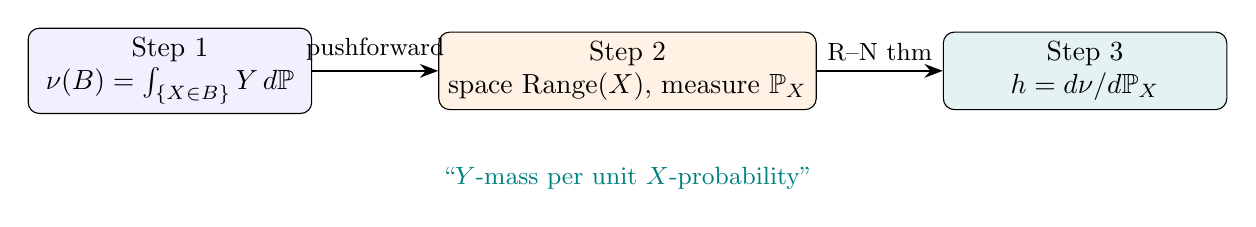
\begin{tikzpicture}[>=Stealth,node distance=1.3cm]
  \node[draw,fill=blue!6,rounded corners,
        minimum width=3.6cm,minimum height=0.9cm,align=center] (s1)
    {Step 1\\$\nu(B)=\int_{\{X\in B\}}Y\,d\Prob$};
  \node[draw,fill=orange!10,rounded corners,
        minimum width=3.6cm,minimum height=0.9cm,align=center,
        right=1.6cm of s1] (s2)
    {Step 2\\space $\Range(X)$, measure $\Prob_X$};
  \node[draw,fill=teal!10,rounded corners,
        minimum width=3.6cm,minimum height=0.9cm,align=center,
        right=1.6cm of s2] (s3)
    {Step 3\\$h=d\nu/d\Prob_X$};
  \draw[->,thick] (s1)--(s2) node[midway,above]{\small pushforward};
  \draw[->,thick] (s2)--(s3) node[midway,above]{\small R--N thm};
  \node[below=0.6cm of s2,teal,align=center]
    {\small ``$Y$-mass per unit $X$-probability''};
\end{tikzpicture}
\end{center}

\begin{definition}[R--N regression function of $Y$ on $X$
  w.r.t.\ $\Prob$]\label{def:RN}
$h:\R\to\R$ is the \emph{R--N regression function of $Y$ on $X$
w.r.t.\ $\Prob$} if
\[
  \int_{\{X\in B\}}Y\,d\Prob = \int_B h\,d\Prob_X
  \qquad\forall\,B\in\borel(\R),
\]
i.e.\ $h=d\nu/d\Prob_X$ where $\nu(B):=\int_{\{X\in B\}}Y\,d\Prob$.
\end{definition}

\begin{remark}[Full name: regression of $Y$ on $X$ w.r.t.\ $\Prob$]
\textbf{Of $Y$}: $Y$ is being averaged.
\textbf{On $X$}: conditioning on the value of $X$; $h$ lives on
$\Range(X)$.
\textbf{W.r.t.\ $\Prob$}: $\Prob$ is the weighting measure;
changing $\Prob$ changes $h$ even if $(X,Y)$ as functions are fixed.
In short: \emph{$h(x)$ is the $\Prob$-average of $Y$ over
$\{\omega:X(\omega)=x\}$}.
\end{remark}

\begin{remark}[Difficulties with signed measures and why $\E|Y|<\infty$
  resolves them]\label{rem:signed}
A natural question arises of whether there are
difficulties in defining a Radon--Nikodym derivative for a signed
measure. The answer is: yes, there are, and the assumption
$\E|Y|<\infty$ is precisely what disposes of them.

\medskip
\textbf{What is a signed measure?}
A signed measure on a measurable space $(\mathcal{X},\mathcal{A})$
is a countably additive set function
$\nu:\mathcal{A}\to[-\infty,+\infty]$ that takes at most one of the
values $\pm\infty$.  The restriction ``at most one'' is necessary to
avoid the indeterminate form $\infty-\infty$ in the additivity
condition.  By the \emph{Hahn decomposition theorem}, $\mathcal{X}$
splits into a positive set $P$ and negative set $N$ (where $\nu$ is
non-negative and non-positive respectively), and one writes
$\nu=\nu^+-\nu^-$ where $\nu^+(B)=\nu(B\cap P)$ and
$\nu^-(B)=-\nu(B\cap N)$ are positive measures.
This is the \emph{Jordan decomposition}, unique up to
$|\nu|:=\nu^++\nu^-$ (the total variation measure).

\medskip
\textbf{The R--N theorem for signed measures and its difficulty.}
If $\nu$ is a signed measure and $\mu$ is a $\sigma$-finite positive
measure with $\nu\ll\mu$, one can formally write
$h=d\nu^+/d\mu - d\nu^-/d\mu$.  The difficulty is
\emph{integrability}: if $\int h^+\,d\mu=+\infty$ and
$\int h^-\,d\mu=+\infty$ simultaneously, then for some sets $B$ the
integral $\int_B h\,d\mu$ is of the form $\infty-\infty$ and is
undefined.  The standard resolution requires at least one of
$\nu^+(\mathcal{X})$ or $\nu^-(\mathcal{X})$ to be finite --- i.e.\
$\nu$ must be a genuine signed measure, not merely a difference of
two infinite positive measures.

\medskip
\textbf{Why there is no difficulty in our setting.}
Our signed measure is $\nu(B)=\int_{\{X\in B\}}Y\,d\Prob$, with
Jordan decomposition $\nu^+(B)=\int_{\{X\in B\}}Y^+\,d\Prob$ and
$\nu^-(B)=\int_{\{X\in B\}}Y^-\,d\Prob$.  The condition
$\E|Y|<\infty$ means:
\[
  \nu^+(\R)=\E Y^+=\int Y^+\,d\Prob<\infty,
  \qquad
  \nu^-(\R)=\E Y^-=\int Y^-\,d\Prob<\infty.
\]
Both are finite, so $\nu$ is a \emph{finite} signed measure, and the
R--N derivative $h=d\nu/d\Prob_X$ is a $\Prob_X$-integrable function
with no $\infty-\infty$ ambiguity.  The assumption $\E|Y|<\infty$ is
not a technicality: it is the exact condition needed to make the
signed measure $\nu$ well-posed.

\medskip
\textbf{References.}
\begin{itemize}[itemsep=2pt]
  \item P.~Halmos, \textit{Measure Theory} (1950), Chapter~VI:
    classical treatment of Hahn and Jordan decompositions.
  \item W.~Rudin, \textit{Real and Complex Analysis}, 3rd ed.\
    (1987), Theorem~6.12: R--N theorem for complex (hence signed)
    measures; finiteness conditions discussed explicitly.
  \item V.~Bogachev, \textit{Measure Theory}, Vol.~1 (2007),
    \S3.10: modern treatment including the $\sigma$-finite case
    and subtleties of the signed setting.
  \item N.~Dunford \& J.T.~Schwartz,
    \textit{Linear Operators}, Vol.~1 (1958), III.7:
    signed measures as elements of the dual of $C_0$;
    functional-analytic perspective.
\end{itemize}
\end{remark}

\begin{theorem}[Existence, uniqueness, properties]\label{thm:RNexist}
Under $\E|Y|<\infty$: $h$ exists; unique $\Prob_X$-a.e.; essential
domain $\mathrm{supp}(\Prob_X)$; $\int h\,d\Prob_X=\E Y$;
$h\in[c,d]$ a.e.\ when $Y\in[c,d]$ a.s.
\end{theorem}

\begin{remark}[Density analogy]
$h$ is an $L^1(\Prob_X)$-equivalence class, free on null sets,
integrating to $\E Y$ --- exactly as probability densities
integrate to $1$.
\end{remark}

\medskip
\begin{center}
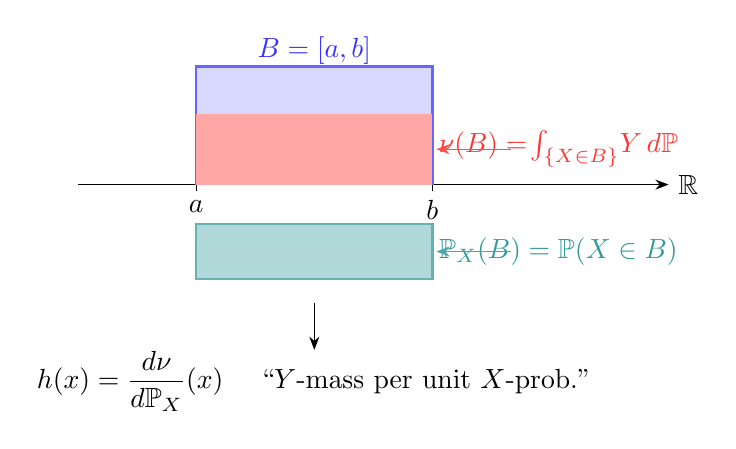
\begin{tikzpicture}[>=Stealth]
  \draw[->] (-0.5,0)--(7,0) node[right]{$\R$};
  \foreach \x/\lbl in {1/$a$,4/$b$}
    \draw(\x,0.08)--(\x,-0.08) node[below]{\lbl};
  \fill[blue!15] (1,0) rectangle (4,1.5);
  \draw[blue!60,thick] (1,0)--(1,1.5)--(4,1.5)--(4,0);
  \node[blue!80] at (2.5,1.7){$B=[a,b]$};
  \fill[red!35] (1,0) rectangle (4,0.9);
  \node[red!80] at (5.6,0.45)
    {$\nu(B)=\!\int_{\{X\in B\}}\!Y\,d\Prob$};
  \draw[->,red!70] (5.0,0.45)--(4.05,0.45);
  \fill[teal!30] (1,-1.2) rectangle (4,-0.5);
  \draw[teal!60,thick] (1,-1.2) rectangle (4,-0.5);
  \node[teal!80] at (5.6,-0.85)
    {$\Prob_X(B)=\Prob(X\in B)$};
  \draw[->,teal!70] (5.0,-0.85)--(4.05,-0.85);
  \draw[->] (2.5,-1.5)--(2.5,-2.1);
  \node at (2.5,-2.5)
    {$h(x)=\dfrac{d\nu}{d\Prob_X}(x)$
     \quad``$Y$-mass per unit $X$-prob.''};
\end{tikzpicture}
\end{center}
\medskip

%------------------------------------------------------------
\subsection{The conditional-expectation regression function}
%------------------------------------------------------------

\begin{definition}[Abstract conditional expectation]\label{def:absCE}
$\E(Y\mid\sG)$ is the unique (up to $\Prob$-a.s.) $\sG$-measurable
r.v.\ with $\int_G\E(Y|\sG)\,d\Prob=\int_G Y\,d\Prob$
for all $G\in\sG$.
\end{definition}

\begin{definition}[C.E.\ regression function of $Y$ on $X$
  w.r.t.\ $\Prob$]\label{def:CEregfun}
Set $Z:=\E(Y\mid\sigma(X))$.  By Doob--Dynkin, $Z=\tilde h(X)$
$\Prob$-a.s.\ for some Borel $\tilde h$.
Any such $\tilde h$ is the \emph{C.E.\ regression function of $Y$
on $X$ w.r.t.\ $\Prob$}.
\end{definition}

\begin{remark}[Role of $\Prob$: R--N vs.\ C.E.]
\begin{center}
\renewcommand{\arraystretch}{1.3}
\begin{tabular}{@{}p{5cm}p{5cm}@{}}
\toprule
\textbf{R--N} & \textbf{C.E.} \\
\midrule
$\Prob$ builds $(\nu,\Prob_X)$, then steps aside.
$h$ lives on $\R$.
& $\Prob$ used throughout on $\Omega$.
$\tilde h$ derived via Doob--Dynkin. \\
Less probabilistic in spirit. & Fundamentally probabilistic. \\
Works for any $\sigma$-finite $\Prob$. & Needs probability structure. \\
\bottomrule
\end{tabular}
\end{center}
\end{remark}

\begin{remark}[Etymology]
``Regression'' from Galton (1886).
Abstract C.E.\ formalised by Kolmogorov (1933).
\end{remark}

\subsection{Equivalence}

\begin{theorem}[$h=\tilde h$ $\Prob_X$-a.e.]\label{thm:equiv}
Any R--N and any C.E.\ regression function agree $\Prob_X$-a.e.
\end{theorem}

\begin{proof}
For any $B$: $\int_B\tilde h\,d\Prob_X
=\int_{\{X\in B\}}Z\,d\Prob
=\int_{\{X\in B\}}Y\,d\Prob=\nu(B)$.
So $\tilde h$ satisfies Def.~\ref{def:RN}; uniqueness gives
$\tilde h=h$ $\Prob_X$-a.e.
\end{proof}

\begin{remark}[Notation]
$\E(Y\mid X=x):=h(x)$ is shorthand only.
\end{remark}

%------------------------------------------------------------
\section{Optimality and the linear projection}
%------------------------------------------------------------

\begin{theorem}[$h$ is the $L^2$-best predictor]\label{thm:l2opt}
Let $Z:=\E(Y\mid X)$ and $U$ be any r.v.\ with
$U\in\sigma(X)$ and $\E U^2<\infty$.  Then
\[
  \E(Y-Z)^2 \;\leq\; \E(Y-U)^2.
\]
Equality holds iff $U=Z$ $\Prob$-a.s.
\end{theorem}

\begin{proof}[Proof ]
Start with the RHS, adding and subtracting $Z$:
\begin{align*}
  \E(Y-U)^2
  &= \E\bigl[(Y-Z)+(Z-U)\bigr]^2 \\
  &= \underbrace{\E(Y-Z)^2}_{=:\,a}
   + \underbrace{2\,\E\bigl[(Y-Z)(Z-U)\bigr]}_{=:\,2b}
   + \underbrace{\E(Z-U)^2}_{=:\,c}.
\end{align*}

\textbf{Step 1: $b=0$.}
Since $Z-U$ is $\sigma(X)$-measurable, pull it out of the
inner conditional expectation using the tower property:
\begin{align*}
  \E\bigl[(Y-Z)(Z-U)\bigr]
  &= \E\Bigl[\E\bigl[(Y-Z)(Z-U)\mid X\bigr]\Bigr] \\
  &= \E\Bigl[(Z-U)\,\E\bigl[Y-Z\mid X\bigr]\Bigr].
\end{align*}
Now $\E[Y-Z\mid X]=\E[Y\mid X]-Z=Z-Z=0$.
Therefore $b=0$.

\textbf{Step 2: $c\geq 0$.}
$c=\E(Z-U)^2\geq 0$ by non-negativity of the square.

Combining: $\E(Y-U)^2=\E(Y-Z)^2+\E(Z-U)^2\geq\E(Y-Z)^2$.
Equality iff $\E(Z-U)^2=0$, i.e.\ $U=Z$ $\Prob$-a.s.
\end{proof}

\begin{remark}[Non-uniqueness as a pointwise function]
The minimiser is not unique as a pointwise function: any
$U$ that equals $Z$ $\Prob$-a.s.\ also achieves the minimum.
The minimiser is unique as a $\Prob$-a.s.\ equivalence class,
or equivalently as an element of $L^2(\Prob)$ (the non-uniqueness argument
from v2 notes).
The key identity in the proof is $\E[Y-Z\mid X]=0$:
this is why the cross-term $b$ vanishes, and this is the
structural role of the conditional expectation.
\end{remark}

%------------------------------------------------------------
\section{The parabola example}
\label{sec:parabola}
%------------------------------------------------------------

\subsection{Setup: a degenerate but instructive case }

The key observation: the parabola example is the most degenerate
possible instance of the R--N construction.

Take:
\[
  (\Omega,\sF,\Prob) = \bigl([0,1],\,\borel([0,1]),\,\Leb\bigr),
  \quad \omega\in[0,1]\subseteq\R.
\]
Define:
\[
  X(\omega) = \omega \quad (\text{identity map}),
  \qquad
  Y(\omega) = (X(\omega))^2 = \omega^2 = h(X(\omega)).
\]

Two key degeneracies follow immediately:

\begin{enumerate}[label=(\arabic*)]
  \item $X(\omega)=\mathrm{id}$, so the event
    $\{X\in B\}=\{\omega:X(\omega)\in B\}=B$.

  \item $\Prob=\Leb$ and $X=\mathrm{id}$, so the pushforward
    $\Prob_X=\Leb$ as well: for any $B$,
    $\Prob_X(B)=\Prob(X\in B)=\Prob(\omega\in B)=\Leb(B)$.
    Thus $\Prob=\Prob_X$ in this example.
\end{enumerate}

\begin{center}
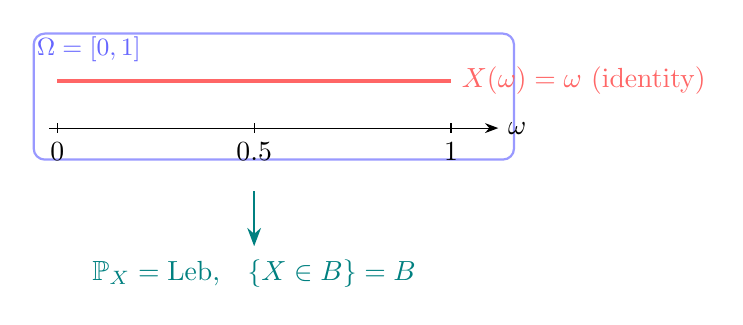
\begin{tikzpicture}[>=Stealth,scale=1.0]
  \draw[blue!40,thick,rounded corners]
    (-0.3,-0.4) rectangle (5.8,1.2);
  \node[blue!60] at (0.4,1.0){\small $\Omega=[0,1]$};

  \draw[->] (-0.1,0)--(5.6,0) node[right]{$\omega$};
  \foreach \x/\lbl in {0/0,2.5/0.5,5/1}
    \draw(\x,0.06)--(\x,-0.06) node[below]{\lbl};

  \draw[red!60,very thick,domain=0:5,samples=2]
    plot({\x},{0.6}) node[right]{$X(\omega)=\omega$ (identity)};

  \draw[->,thick,teal] (2.5,-0.8)--(2.5,-1.5);
  \node[teal] at (2.5,-1.85)
    {$\Prob_X = \Leb$,\quad $\{X\in B\}=B$};
\end{tikzpicture}
\end{center}

\subsection{The R--N construction collapses to a trivial density}

With $\{X\in B\}=B$ and $\Prob=\Leb$:
\[
  \nu(B) = \int_{\{X\in B\}} Y\,d\Prob
         = \int_B \omega^2\,d\omega
         = \int_B x^2\,dx.
\]
Reference measure: $\Prob_X=\Leb$.
R--N density: $h = d\nu/d\Leb = x^2$.

There is no averaging taking place: $Y$ is a deterministic function
of $X$ (in fact $Y=h\circ X$ by construction), so $h$ simply reads
off the value of $Y$ at each $x$.  The regression function is
trivial precisely because there is no randomness in $Y$ given $X$.

\begin{remark}[Why this is the degenerate case]
In a general regression problem, $Y$ is not determined by $X$:
for the same $x$ there is a distribution of $Y$-values, and $h(x)$
averages them.  Here the ``distribution of $Y$ given $X=x$'' is the
point mass at $x^2$, so the average is $x^2$ itself.

This is made precise as follows: since $X=\mathrm{id}$ and
$\Prob=\Prob_X$, the three-step construction (Remark~\ref{rem:verbalization})
degenerates:
\begin{itemize}
  \item $\nu(B)=\int_B x^2\,dx$ (direct integral, no ``restriction'' needed),
  \item $\Prob_X=\Leb=\Prob$ (no pushforward needed),
  \item $h=x^2$ (density of $x^2\,dx$ w.r.t.\ $dx$, i.e.\ just $x^2$).
\end{itemize}
\end{remark}

\subsection{The affine projection $\ell^*$}

Minimise $f(a,b)=\int_0^1(x^2-(a+bx))^2\,dx$:
\[
  f(a,b)
  =\tfrac{1}{5}-\tfrac{2a}{3}-\tfrac{b}{2}+a^2+ab+\tfrac{b^2}{3}.
\]
(Coefficient of $b$ is $-\tfrac{1}{2}$: the notes had a
factor-of-2 error.)
First-order conditions give $a=-\tfrac{1}{6}$, $b=1$:
\[
  \boxed{\ell^*(x) = -\tfrac{1}{6}+x.}
\]

\medskip
\begin{center}
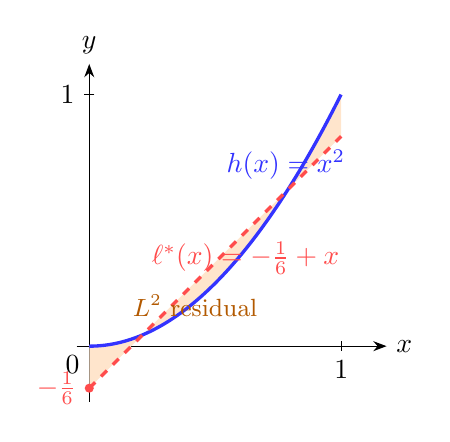
\begin{tikzpicture}[>=Stealth,scale=3.2]
  \draw[->] (-0.05,0)--(1.18,0) node[right]{$x$};
  \draw[->] (0,-0.22)--(0,1.12) node[above]{$y$};
  \fill[orange!20,domain=0:1,samples=80,variable=\x]
    (0,0)--plot({\x},{\x*\x})--(1,1)--
    plot[domain=1:0]({\x},{-1/6+\x})--cycle;
  \draw[blue!80,very thick,domain=0:1,samples=80]
    plot({\x},{\x*\x});
  \node[blue!80] at (0.78,0.72){$h(x)=x^2$};
  \draw[red!70,very thick,dashed,domain=0:1]
    plot({\x},{-1/6+\x});
  \node[red!70] at (0.62,0.35){$\ell^*(x)=-\tfrac{1}{6}+x$};
  \draw(1,0.02)--(1,-0.02) node[below]{$1$};
  \draw(0.02,1)--(-0.02,1) node[left]{$1$};
  \node at (0,0)[below left]{$0$};
  \node[orange!70!black] at (0.42,0.16){\small $L^2$ residual};
  \fill[red!70] (0,-1/6) circle(0.018);
  \node[red!70] at (-0.13,-1/6){$-\tfrac{1}{6}$};
\end{tikzpicture}
\end{center}
\medskip

\subsection{Three objects and the GLM}

\begin{center}
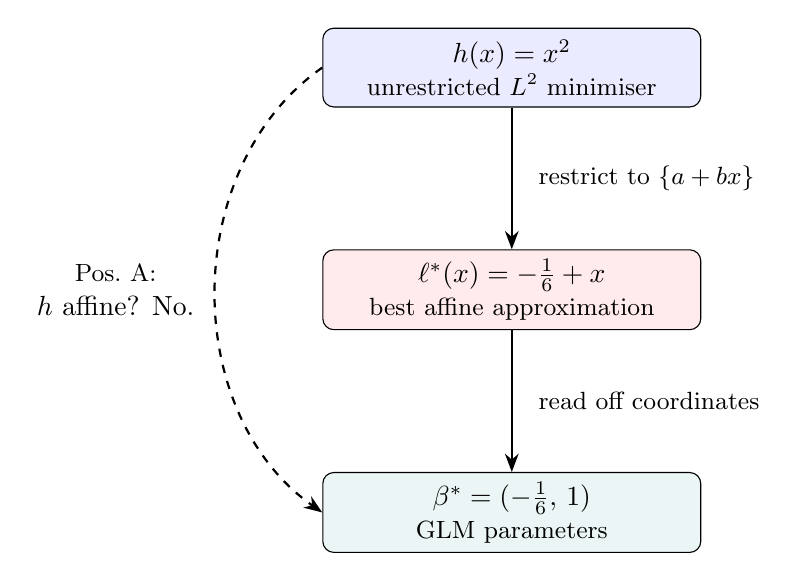
\begin{tikzpicture}[>=Stealth,node distance=1.6cm]
  \node[draw,rounded corners,fill=blue!8,
        minimum width=4.8cm,minimum height=1.0cm,align=center] (h)
    {$h(x)=x^2$\\{\small unrestricted $L^2$ minimiser}};
  \node[draw,rounded corners,fill=red!8,
        minimum width=4.8cm,minimum height=1.0cm,align=center,
        below=1.8cm of h] (ell)
    {$\ell^*(x)=-\tfrac{1}{6}+x$\\
     {\small best affine approximation}};
  \node[draw,rounded corners,fill=teal!8,
        minimum width=4.8cm,minimum height=1.0cm,align=center,
        below=1.8cm of ell] (beta)
    {$\beta^*=(-\tfrac{1}{6},\,1)$\\{\small GLM parameters}};
  \draw[->,thick](h)--(ell)
    node[midway,right=6pt]{\small restrict to $\{a+bx\}$};
  \draw[->,thick](ell)--(beta)
    node[midway,right=6pt]{\small read off coordinates};
  \draw[->,thick,dashed,bend right=55]
    (h.west) to node[left=4pt,align=center]
      {\small Pos.\ A:\\$h$ affine? No.}
    (beta.west);
\end{tikzpicture}
\end{center}

\begin{remark}[Positions A and B]
\textbf{A}: requires $h=x^2$ to be affine --- false here.
\textbf{B}: $\beta^*=(-\tfrac{1}{6},1)$ are best-approximation
parameters; estimating them is meaningful even under misspecification.
\end{remark}

%------------------------------------------------------------
\section{The underspecification argument}
%------------------------------------------------------------

\begin{remark}[Free $g$ is vacuous; fixing $g$ is substantive]
If $h$ injective: set $g=h^{-1}$, $\beta_0=0$, $\beta_1=1$.
Any injective $h$ satisfies the GLM equation.
Fixing $g$ is a genuine modelling commitment.
\end{remark}

\begin{assumption}[Position A]
$h(x)=g^{-1}(\beta_0^*+\beta_1^*x)$ $\Prob_X$-a.e.
MLE consistent and asymptotically normal.
\end{assumption}

\begin{remark}[Position B]
$\beta^*=\operatorname{argmin}\E[Y-g^{-1}(b_0+b_1X)]^2$.
MLE$\to\beta^*$; sandwich s.e.\ valid (White 1982).
Quasi-likelihood (Wedderburn 1974): correct two moments suffice.
\end{remark}

%------------------------------------------------------------
\section{The GLM framework}
%------------------------------------------------------------

Three components: (i) exponential family $\mu=b'(\theta)$;
(ii) $\eta=\mathbf{x}^\top\boldsymbol\beta$;
(iii) link $g(\mu)=\eta$, canonical: $g=(b')^{-1}$.

\begin{center}
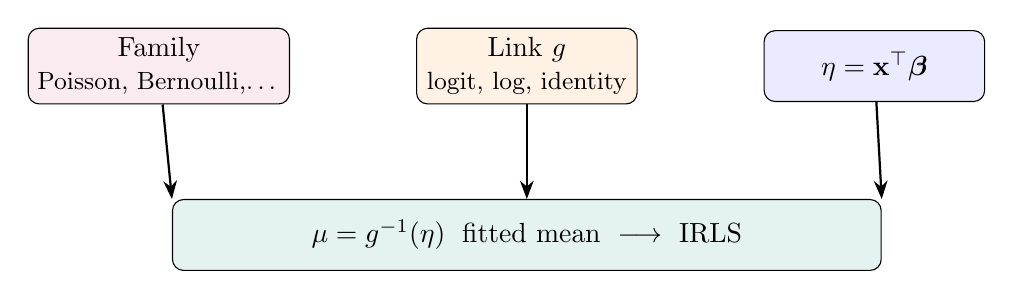
\begin{tikzpicture}[>=Stealth,node distance=1.1cm]
  \node[draw,fill=purple!8,rounded corners,
        minimum width=2.8cm,minimum height=0.9cm,align=center] (fam)
    {Family\\{\small Poisson, Bernoulli,\ldots}};
  \node[draw,fill=orange!10,rounded corners,
        minimum width=2.8cm,minimum height=0.9cm,align=center,
        right=1.6cm of fam] (link)
    {Link $g$\\{\small logit, log, identity}};
  \node[draw,fill=blue!8,rounded corners,
        minimum width=2.8cm,minimum height=0.9cm,align=center,
        right=1.6cm of link] (lin)
    {$\eta=\mathbf{x}^\top\boldsymbol\beta$};
  \node[draw,fill=teal!10,rounded corners,
        minimum width=9cm,minimum height=0.9cm,align=center,
        below=1.2cm of link] (mu)
    {$\mu=g^{-1}(\eta)$ \;fitted mean\;
     $\longrightarrow$ \;IRLS};
  \draw[->,thick](fam)--(mu.north west);
  \draw[->,thick](link)--(mu);
  \draw[->,thick](lin)--(mu.north east);
\end{tikzpicture}
\end{center}

\begin{table}[h]
\centering
\caption{Canonical links.}
\renewcommand{\arraystretch}{1.4}
\begin{tabular}{lllll}
\toprule
Family & Support & $b(\theta)$ & Canonical $g(\mu)$ & $V(\mu)$ \\
\midrule
Gaussian  & $\R$ & $\theta^2/2$ & $\mu$ & $1$ \\
Bernoulli & $\{0,1\}$ & $\log(1+e^\theta)$ & $\logit(\mu)$ & $\mu(1-\mu)$ \\
Poisson   & $\mathbb{Z}_{\geq0}$ & $e^\theta$ & $\log\mu$ & $\mu$ \\
Gamma     & $(0,\infty)$ & $-\log(-\theta)$ & $-1/\mu$ & $\mu^2$ \\
Inv.\ Gauss & $(0,\infty)$ & $-\sqrt{-2\theta}$ & $1/\mu^2$ & $\mu^3$ \\
\bottomrule
\end{tabular}
\end{table}

%------------------------------------------------------------
\section{Logistic regression: Bernoulli case}
%------------------------------------------------------------

\subsection{Conditional probability for continuous $X$}

\begin{center}
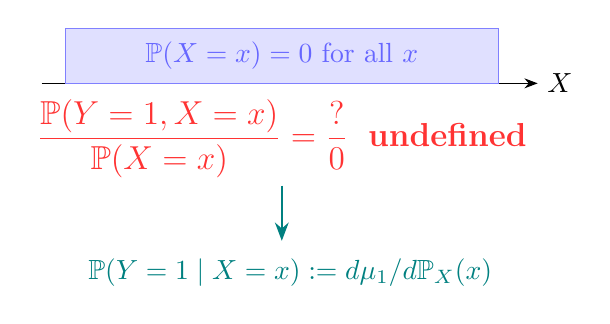
\begin{tikzpicture}[>=Stealth]
  \draw[->](-0.3,0)--(6,0) node[right]{$X$};
  \fill[blue!12](0,0) rectangle (5.5,0.7);
  \draw[blue!50](0,0) rectangle (5.5,0.7);
  \node[blue!60] at (2.75,0.35)
    {$\Prob(X=x)=0$ for all $x$};
  \node[red!80,font=\large] at (2.75,-0.7)
    {$\dfrac{\Prob(Y=1,X=x)}{\Prob(X=x)}=\dfrac{?}{0}$
     \;\textbf{undefined}};
  \draw[->,thick,teal](2.75,-1.3)--(2.75,-2.0);
  \node[teal,align=center] at (2.75,-2.4)
    { \;
     $\Prob(Y=1\mid X=x):=d\mu_1/d\Prob_X(x)$};
\end{tikzpicture}
\end{center}

\begin{definition}[$\Prob(Y=1\mid X=x)$ via R--N]\label{def:condprob}
$\mu_1(B):=\Prob(Y=1,X\in B)$. Then $\mu_1\ll\Prob_X$ and
$\Prob(Y=1\mid X=x):=d\mu_1/d\Prob_X(x)$.
Recovers elementary ratio for discrete $X$.
\end{definition}

\begin{proposition}\label{prop:bern}
For $Y\in\{0,1\}$: $h(x)=\Prob(Y=1\mid X=x)$ $\Prob_X$-a.e.
\end{proposition}
\begin{proof}
Both are R--N derivatives of $\mu_1$ w.r.t.\ $\Prob_X$.
\end{proof}

\subsection{The logistic model}

\begin{center}
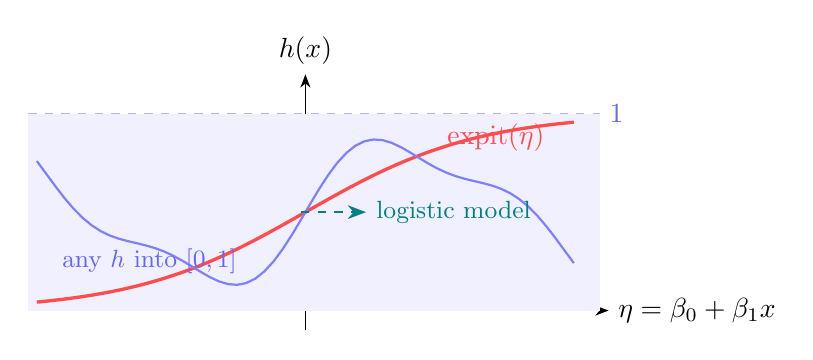
\begin{tikzpicture}[>=Stealth]
  \begin{scope}[xscale=1.1,yscale=2.5]
    \draw[->](-3.2,0)--(3.5,0)
      node[right]{$\eta=\beta_0+\beta_1 x$};
    \draw[->](0,-0.1)--(0,1.2) node[above]{$h(x)$};
    \fill[blue!6](-3.2,0) rectangle (3.4,1);
    \draw[blue!30,dashed](-3.2,1)--(3.4,1)
      node[right,blue!60]{$1$};
    \draw[red!70,very thick,domain=-3.1:3.1,samples=100]
      plot({\x},{1/(1+exp(-\x))});
    \node[red!70] at (2.2,0.88){$\expit(\eta)$};
    \draw[blue!50,thick,domain=-3.1:3.1,samples=60]
      plot({\x},{0.5+0.35*sin(deg(\x*1.3))
                    +0.1*sin(deg(\x*3))});
    \node[blue!60] at (-1.8,0.25){\small any $h$ into $[0,1]$};
    \draw[->,thick,teal,dashed](-0.05,0.5)--(0.7,0.5)
      node[right,teal]{\small logistic model};
  \end{scope}
\end{tikzpicture}
\end{center}

Range condition necessary but not sufficient.
Logistic model restricts to the parametric family
$\{\expit(\beta_0+\beta_1\cdot):(\beta_0,\beta_1)\in\R^2\}$.

%------------------------------------------------------------
\section{IRLS}
%------------------------------------------------------------

Score equations: $\mathbf{X}^\top\mathbf{W}\mathbf{D}
(\mathbf{y}-\boldsymbol\mu)=\mathbf{0}$,
$W_{ii}=[V(\mu_i)(g'(\mu_i))^2]^{-1}$.  Update:
\[
  \boldsymbol\beta^{(t+1)}
  =(\mathbf{X}^\top\mathbf{W}^{(t)}\mathbf{X})^{-1}
   \mathbf{X}^\top\mathbf{W}^{(t)}\mathbf{z}^{(t)},
  \quad
  \mathbf{z}^{(t)}=\mathbf{X}\boldsymbol\beta^{(t)}
    +\mathbf{D}^{(t)}(\mathbf{y}-\boldsymbol\mu^{(t)}).
\]
Logistic: $W_{ii}=\hat p_i(1-\hat p_i)$.
OLS: Gaussian, identity, $W=I$, one step.

%------------------------------------------------------------
\section{Summary}
%------------------------------------------------------------

\begin{enumerate}
  \item \textbf{Atoms} (Lemma~\ref{lem:atoms}): $\sigma(X)$-measurable
    functions are constant a.e.\ on atoms $\{X=x_i\}$; this justifies
    $h(x_i)=\E[Y\mid X=x_i]$ as a single number.

  \item \textbf{Full name}: R--N regression function of $Y$ on $X$
    w.r.t.\ $\Prob$. Three-step construction
    (Remark~\ref{rem:verbalization}). $\Prob$ need not be a
    probability measure.

  \item \textbf{Degenerate parabola case} (degenerate case):
    $(\Omega,\sF,\Prob)=([0,1],\borel([0,1]),\Leb)$,
    $X=\mathrm{id}$, $Y=X^2$. Then $\Prob=\Prob_X$,
    $\{X\in B\}=B$, and the R--N construction gives $h=x^2$
    without any averaging. The regression is trivial because $Y$
    is determined by $X$.

  \item \textbf{Optimality proof} (optimality):
    $\E(Y-Z)^2\leq\E(Y-U)^2$ for all $U\in\sigma(X)$.
    Key: decompose $E(Y-U)^2=a+2b+c$; the cross-term $b=0$ because
    $\E[Y-Z\mid X]=0$; remainder $c\geq 0$.

  \item \textbf{Uniqueness}: $h$ unique as $\Prob_X$-equivalence class,
    not pointwise.

  \item R--N and C.E.\ definitions agree $\Prob_X$-a.e.\
    (Thm.~\ref{thm:equiv}).

  \item Conditional probability for continuous $X$ requires R--N
    ( Binary $Y$: $h=\Prob(Y=1\mid X=\cdot)$.

  \item Canonical links derived via $g=(b')^{-1}$.
\end{enumerate}

%------------------------------------------------------------
\appendix
\section{Notation}
%------------------------------------------------------------
\begin{tabular}{@{}ll@{}}
$(\Omega,\sF,\Prob)$ & probability space \\
$\Prob_X=X_*\Prob$ & pushforward of $X$ \\
$\Range(X)=X(\Omega)$ & essential domain of $h$ \\
$\nu(B)=\int_{\{X\in B\}}Y\,d\Prob$ & signed measure \\
$h=d\nu/d\Prob_X$ & R--N regression fn of $Y$ on $X$ w.r.t.\ $\Prob$ \\
$\tilde h$ & C.E.\ regression function \\
$Z=\E(Y\mid X)$ & conditional expectation r.v. \\
$\E(Y\mid X=x):=h(x)$ & notation only \\
$\ell^*(x)$ & best affine approx.\ to $h$ \\
$\mu_1(B)=\Prob(Y=1,X\in B)$ & Bernoulli measure \\
$g$ & link function (fixed) \\
$b(\theta)$ & log-partition function \\
$V(\mu)$ & variance function \\
$\expit$, $\logit$ & logistic and logit \\
IRLS & iteratively reweighted least squares \\
R--N & Radon--Nikodym \\
\end{tabular}

\end{document}
